\begin{figure}[h]
    \centering
    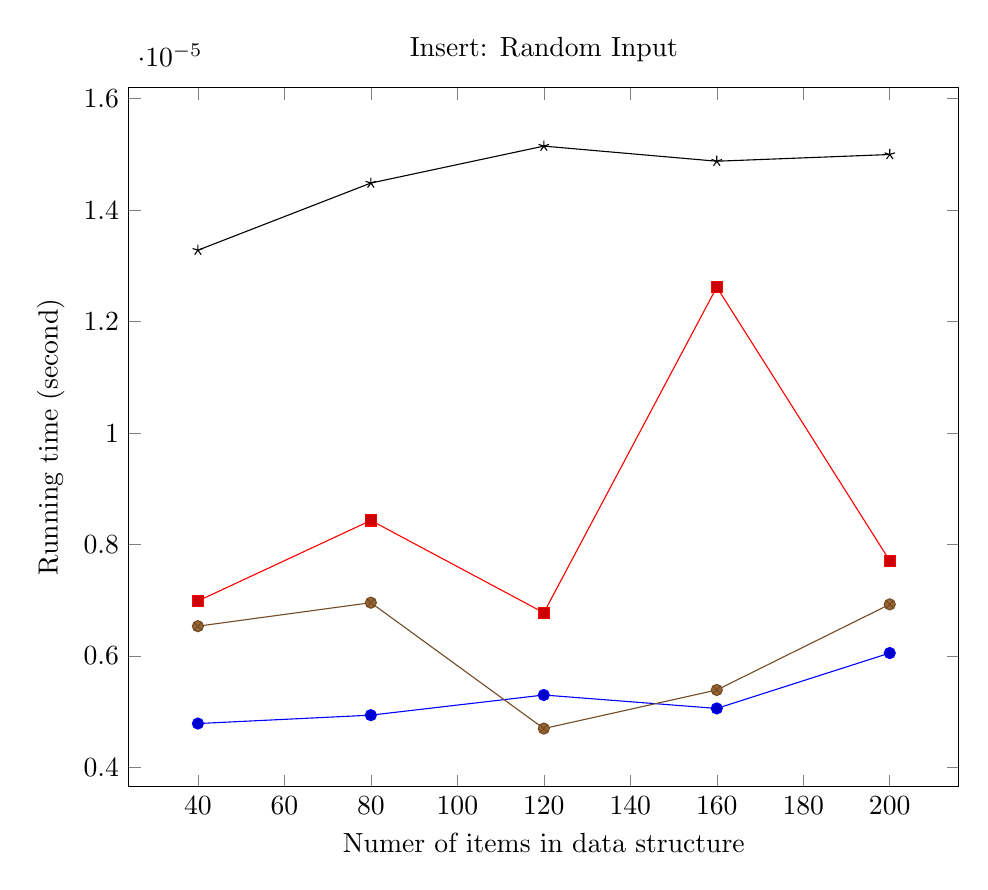
\begin{tikzpicture}
        \begin{axis}[
            xlabel={Numer of items in data structure},
            ylabel={Running time (second)},
            title={Insert: Random Input},
            width=\textwidth
        ]
		\addplot coordinates {
			(40, 4.78868785435127e-06)
			(80, 4.939275522727882e-06)
			(120, 5.300685926828974e-06)
			(160, 5.0597456574263955e-06)
			(200, 6.0536242687092566e-06)
		};
		\addplot coordinates {
			(40, 6.987267812638698e-06)
			(80, 8.432909429048618e-06)
			(120, 6.776445076911442e-06)
			(160, 1.2619246609896218e-05)
			(200, 7.710088620843657e-06)
		};
		\addplot coordinates {
			(40, 6.535504807508863e-06)
			(80, 6.957150278963376e-06)
			(120, 4.698335253328079e-06)
			(160, 5.391038527854941e-06)
			(200, 6.9270327452880535e-06)
		};
		\addplot coordinates {
			(40, 1.3281832350747758e-05)
			(80, 1.44865336977551e-05)
			(120, 1.5149119438609416e-05)
			(160, 1.487806163553429e-05)
			(200, 1.4998531770232804e-05)
		};
        \legend{}
        \end{axis}
    \end{tikzpicture}
    \caption{Average of 0 operations, benchmarked every 0, starting at 0.}
\end{figure}